\documentclass{article}
\usepackage[utf8]{inputenc}

% --- Language and Font Fix ---
% The 'babel' package is the standard way to handle multilingual documents.
% It automatically selects the correct fonts and hyphenation patterns.
% [english, vietnamese] sets English as the main language and allows switching to Vietnamese.
% This replaces the need for manual \usepackage[T5]{fontenc}.
\usepackage[english, vietnamese]{babel} 

\usepackage{amsmath, amsfonts, amssymb} % For mathematical equations and symbols
\usepackage{graphicx} % For including images
\usepackage{geometry} % For page layout
\geometry{a4paper, margin=1in} % Set page margins
\usepackage{tabularx} % For flexible table columns
\usepackage{enumitem} % For custom list environments
\usepackage{hyperref} % For clickable links in the table of contents
% --- Corrected Custom Commands for Vietnamese Text ---
% Use \foreignlanguage{vietnamese}{...} to correctly typeset Vietnamese text.
% This command is provided by the 'babel' package.
\newcommand{\vietnameseuniversity}{\foreignlanguage{vietnamese}{ĐẠI HỌC BÁCH KHOA HÀ NỘI}}
\newcommand{\vietnameseschool}{\foreignlanguage{vietnamese}{TRƯỜNG CÔNG NGHỆ THÔNG TIN VÀ TRUYỀN THÔNG}}

\begin{document}

% --- Title Page/Header ---
\begin{titlepage}
    \centering
    % You might want to include the university logo here
    % Make sure the file 'hust_logo.png' is in the same directory
    \includegraphics[width=0.3\textwidth]{logo.png} 
    
    \vspace{1cm}
    
    {\Huge \vietnameseuniversity \par}
    \vspace{0.25cm}
    {\Large \vietnameseschool \par}
    
    \vspace{2cm}
    
    {\Huge \textbf{Report} \par}
    \vspace{0.5cm}
    {\Huge \textbf{Effects of superspreaders in spread of epidemic} \par}
    
    \vspace{2.5cm}

    % Using a simple tabular for alignment.
    % Also wrapped Vietnamese names with \foreignlanguage for correctness.
    \begin{tabular}{l l l}
        \textbf{Student name} & : & \foreignlanguage{vietnamese}{Phạm Anh Tú} \\
        \textbf{Student ID}   & : & 20225463 \\
        \textbf{Class}        & : & 157209 \\
        \textbf{Course}       & : & Mathematical Modeling \\
        \textbf{Course ID}    & : & IT4033E \\
        \textbf{Teacher}      & : & \foreignlanguage{vietnamese}{Bùi Quốc Trung} \\
    \end{tabular}
    
    \vfill % Pushes the date to the bottom of the page
    
    {\large \textit{\foreignlanguage{vietnamese}{Hà Nội}, 24th May 2025} \par}
\end{titlepage}

\clearpage

% --- Table of Contents ---
\tableofcontents
\clearpage

% --- I. INTRODUCTION ---
\section{INTRODUCTION}
Analyzing infectious disease dynamics is crucial for public health, enabling outbreak predictions and the evaluation of control measures. Traditional epidemiological models often simplify population characteristics, assuming homogeneity in factors like infectiousness and contact rates. However, real-world epidemics are frequently characterized by significant heterogeneity, where a small number of individuals contribute disproportionately to transmission. These individuals, known as "superspreaders," can drive "superspreading events" (SSEs) that dramatically accelerate and widen the scope of an outbreak. The 2003 SARS (Severe Acute Respiratory Syndrome) epidemic prominently featured such events, highlighting the need for models that can account for this phenomenon.

The reference paper, "Effects of superspreaders in spread of epidemic" by Ryo Fujie and Takashi Odagaki (2007), directly addresses this challenge. It aims to investigate the impact of superspreaders by proposing and simulating two distinct mechanisms for superspreading behavior within a spatial Susceptible-Infected-Recovered (SIR) framework. This report will review the modeling approach, mathematical formulation, simulation algorithm, and key conclusions presented by Fujie and Odagaki. Furthermore, it will discuss the model's sensitivity and robustness, potentially drawing insights from a Python implementation of these models.

% --- II. MODELING APPROACH ---
\section{MODELING APPROACH}
Fujie and Odagaki (2007) started from a standard Susceptible-Infected-Recovered (SIR) model analysis, but with some significant additions to allow for the complexities of superspreading.

Their key modeling elements are :
\begin{itemize}[leftmargin=*, align=left]
    \item \textbf{Spatial Structure}: The subjects (N total) are spread in a continuous two-dimensional space of size L x L with fixed positions. Periodic boundary conditions are implemented to minimize edge effects. This spatial structure allows distance-dependent interactions to be specified, beyond the mean-field assumptions of non-spatial compartmental models.
    \item \textbf{Distance-Dependent Infection Probability (\(w(r)\))}: The infection probability of a susceptible person by an infected person is a function of the Euclidean distance \(r\) separating the two. This captures the intuitive notion that contacts between people who are in close proximity to each other are more likely to lead to infection.
    \item \textbf{Two Distinct Superspreader Models}: To explore other underlying mechanisms for superspreading, the authors proposed two hypotheses, which were implemented as two alternate models for superspreader individuals (who comprise a fraction \(\lambda\) of the population) :
    \begin{itemize}
        \item \textbf{Strong Infectiousness Model}: Superspreaders simply have a higher probability of infecting others within the same interaction radius (cutoff distance \(r_0\)) as normal individuals.
        \item \textbf{Hub Model}: Superspreaders are characterized as having a vastly larger interaction range than normal people. This represents individuals with more social contacts or opportunities to transmit the disease over long distances, even if their intrinsic infectiousness profile within that range is identical to normal people.
    \end{itemize}
\end{itemize}
This modeling approach was chosen to better approximate the spread of epidemics in the real world. The SIR model needed generalization to represent the differential impact of superspreaders. While more complex network models exist, the authors chose a "simplified model" that still incorporated essential elements like spatiality and distance to directly investigate superspreader mechanisms. Their ultimate goal was to see if these simplified models could reproduce observed phenomena in the SARS epidemic.

% --- III. MATHEMATICAL MODELING ---
\section{MATHEMATICAL MODELING}
N individuals are randomly placed (except for the initial infector) with fixed positions \(p_i\) in an L x L continuous space with periodic boundary conditions. Each individual \(i\) can be in one of three states at a given time step \(t\): susceptible (S), infected (I), or recovered (R). Initially, there are N - 1 susceptible individuals and 1 infected. Infected individuals can turn to recovered state with probability \(\gamma\). Initially, there are exactly \(\lfloor \lambda N \rfloor\) superspreaders.

Since we are using periodic boundary conditions, the distance of two individuals \(i\) and \(j\) is given by :
\[
r = d(i, j) = \sqrt{\sum_k \min(|p_{i, k} - p_{j, k}|, L - |p_{i, k} - p_{j, k}|)^2}
\]
The probability of an infected individual at \(p_j\) infecting a susceptible individual at \(p_i\) at distance \(r\) within one Monte Carlo step is :
\[
w(r) = w_0 \cdot \left(1 - \frac{r}{r_0}\right)^\alpha \quad \text{for } 0 < r \le r_0
\]
\[
w(r) = 0 \quad \text{for } r > r_0
\]
In the strong infectious model, \(\alpha\) is equal to 0 for superspreaders, meaning a susceptible individual in range \(r_0\) with an infected individual is guaranteed to be infected. For normal individuals, \(\alpha\) is set to 2.

In the hub model, superspreaders make more contact with other people, so their cutoff distance is longer. Specifically, a superspreader cutoff distance is \(r_n = \sqrt{6} \cdot r_0\).
\[
w(r) = w_0 \cdot \left(1 - \frac{r}{r_n}\right)^2 \quad \text{for } 0 < r \le r_n
\]
\[
w(r) = 0 \quad \text{for } r > r_n
\]
where \(r_n = \sqrt{6} \cdot r_0\).

% --- IV. SOLVING ALGORITHM ---
\section{SOLVING ALGORITHM}
The solving algorithm used in the reference paper is Monte Carlo simulation. The simulation was run 1000 times with different initial positions, and the average of some quantities was logged. They used the following parameter settings :
\begin{itemize}
    \item \(N\) in range 150 to 900
    \item \(L = 10r_0\)
    \item \(w_0 = 1\)
    \item \(\gamma = 1\)
\end{itemize}
In our experiments, we lower the number of simulation runs to 100 and modify our parameter settings to better suit our computational resources :
\begin{itemize}
    \item \(N = 200\)
    \item \(L = \sqrt{\frac{N \cdot \pi \cdot r_0^2}{\text{density}}}\)
    \item Density in range 0 to 25
\end{itemize}

% --- V. RESULTS ---
\section{RESULTS}
\subsection{Percolation probability}
The original paper defined percolation as the event when the infection started at the bottom of the system reaches on the top of it. The percolation probability is then defined as the fraction of runs in which percolation occurs. The paper did not provide definitions of "bottom" and "top" of the system, so we assume that bottom is the state with only one infected individual and top is the state where all individuals are infected. 

Replicating the experiment with our parameter settings, we achieve similar results. Figure \ref{fig:percolation_probability} shows the function of percolation probability on several values of \(\lambda\) (superspreader fraction) for both Strong Infectiousness and Hub Models. In the case of no superspreader (\(\lambda\ = 0\), the infection rarely reach the top state. As \(\lambda\) increases, the percolation probability also rapidly increases at lower density values.

\begin{figure}[!htbp]
    \centering
    % Placeholder for the third image (two subplots)
    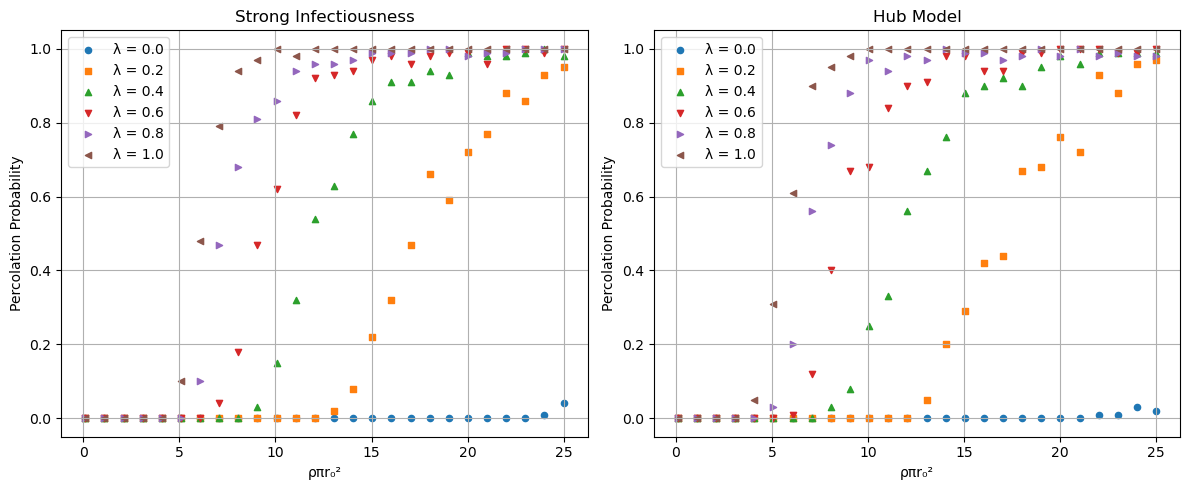
\includegraphics[width=0.9\textwidth]{fig/percolation.png} % Replace with your image file
    % \fbox{\parbox[c][5cm][c]{0.9\textwidth}{\centering \textit{Placeholder for "Percolation Probability" plot.} \\ Two subplots: "Strong Infectiousness" (left) and "Hub Model" (right). \\ X-axis: \( \rho\pi r_0^2 \). Y-axis: Percolation Probability. \\ Multiple lines with different markers represent varying values of \(\lambda\) (superspreader fraction): 0.0, 0.2, 0.4, 0.6, 0.8, 1.0.}}
    \caption{Percolation probability as a function of \(\rho\pi r_0^2\) for both Strong Infectiousness and Hub Models, demonstrating the effect of different superspreader fractions \(\lambda\).}
    \label{fig:percolation_probability}
\end{figure}

\subsection{Propagation velocity}
The paper defined the velocity of propagation as the velocity of front line. Let \(r_f\) be the distance between the initial infected individual and the furthest infected individual. The velocity is then defined as:
\[
\frac{r_f}{r_0 \cdot t}
\]
where \(t\) is the time step when the furthest infected individual is reached. We calculate the average propagation velocity as the average of velocities over all runs. As shown in figure \ref{fig:propagation_speed}, the propagation velocity of the hub model is consistently larger than that of the strong infectiousness model. 
\begin{figure}[!htbp]
    \centering
    % Placeholder for the fourth image
    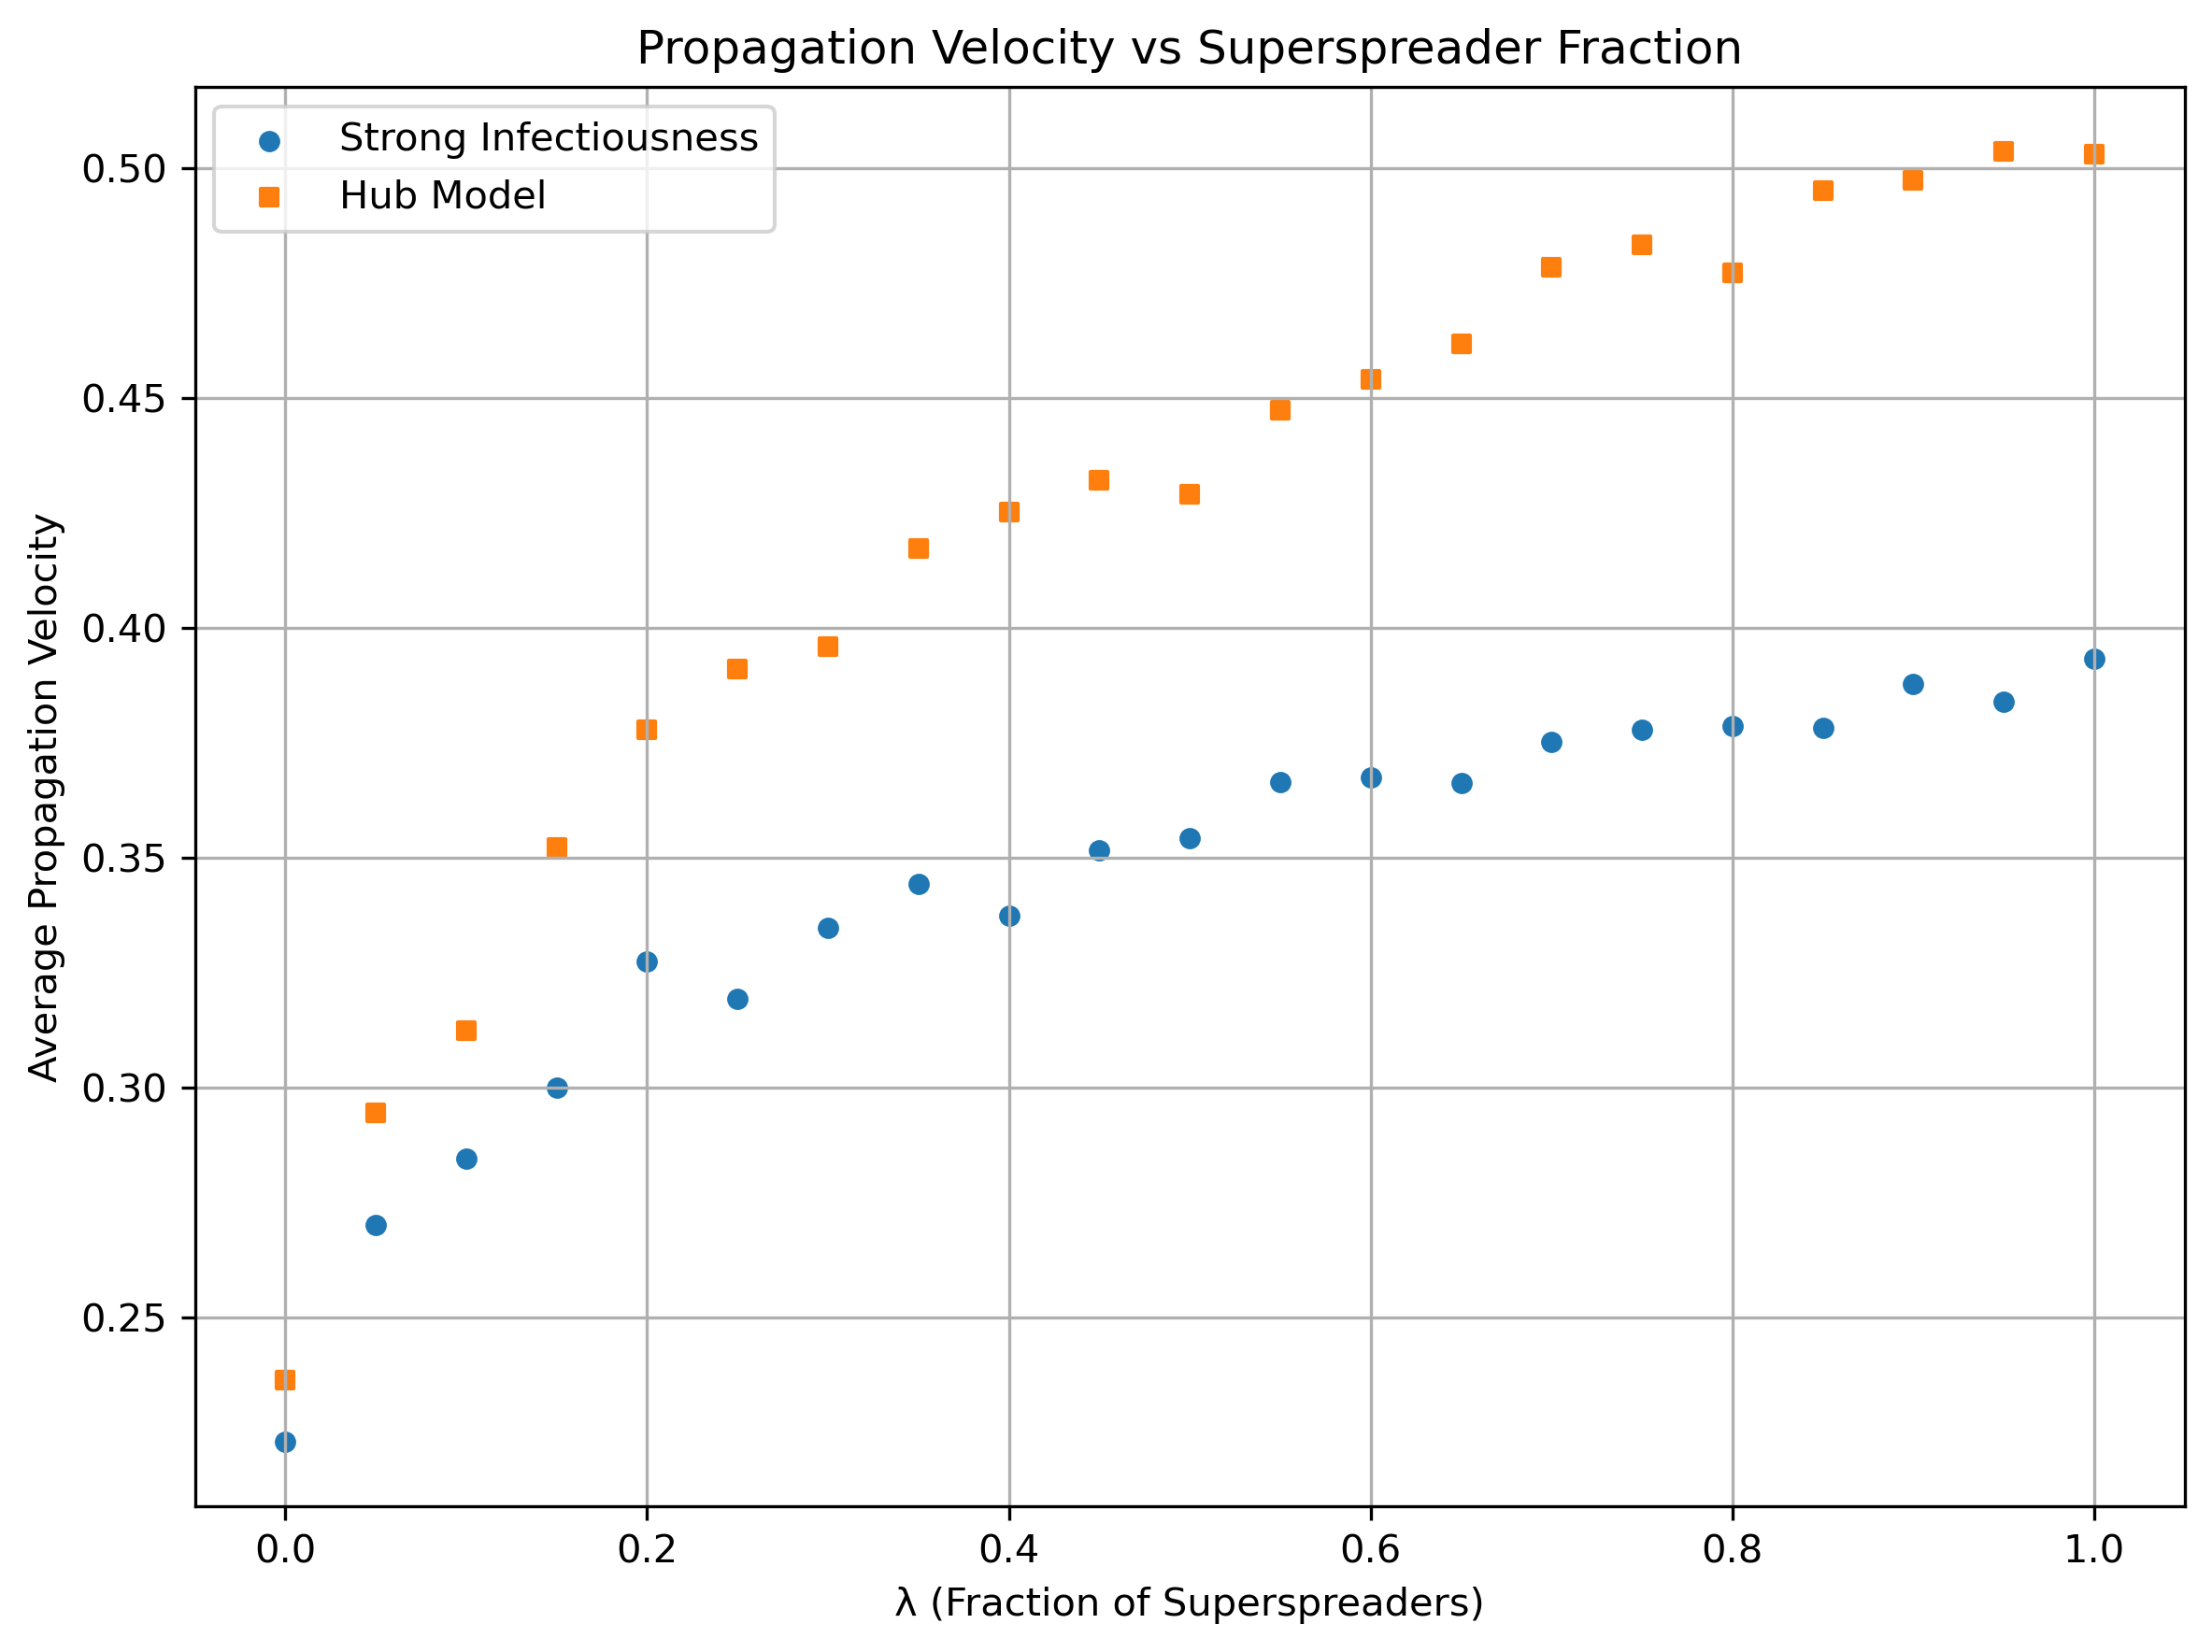
\includegraphics[width=0.8\textwidth]{fig/velocity.png} % Replace with your image file
    \caption{Average Propagation Velocity versus the fraction of superspreaders (\(\lambda\)) for both Strong Infectiousness and Hub Models.}
    \label{fig:propagation_speed}
\end{figure}

\subsection{Infection Distribution}
We visualize each step of the simulation to see how the infected individuals are distributed on the LxL space. Figures \ref{fig:side_by_side_snapshots_1}, \ref{fig:side_by_side_snapshots_2}, \ref{fig:side_by_side_snapshots_3} compare the two models in each time step for a short simulation. A common trend we found is that infected individuals in the hub model are more spread out than in the strong infectious model. However, strong infectious model does prolong the epidemic longer thanks to the guaranteed infectiousness, which we will investigate further in the next section.

\begin{figure}[!htbp]
    \centering
    \begin{tabular}{cc}
        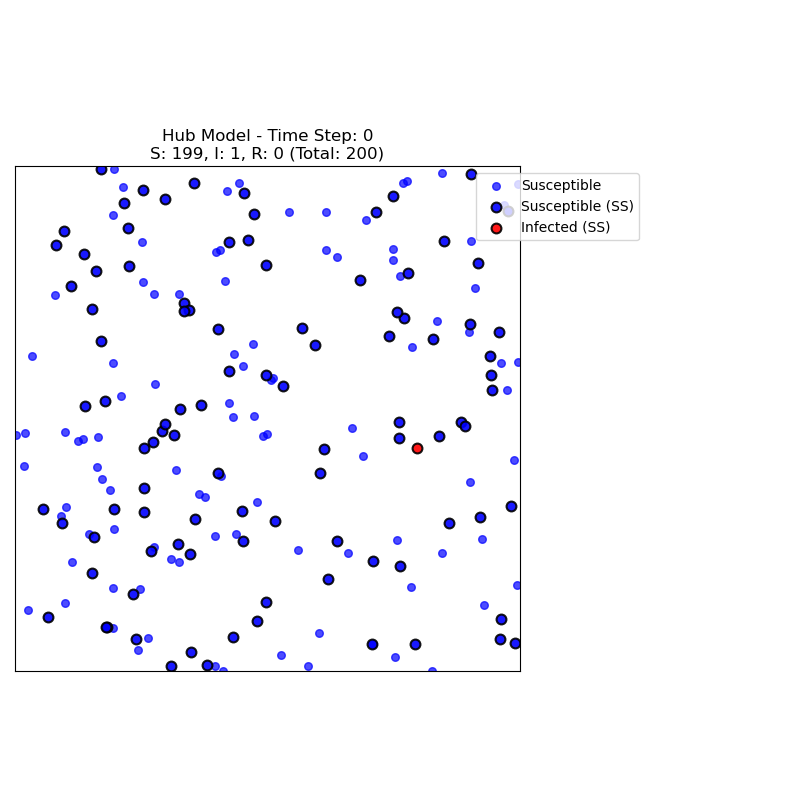
\includegraphics[width=0.4\textwidth]{fig/sir_hub_step_0.png} &
        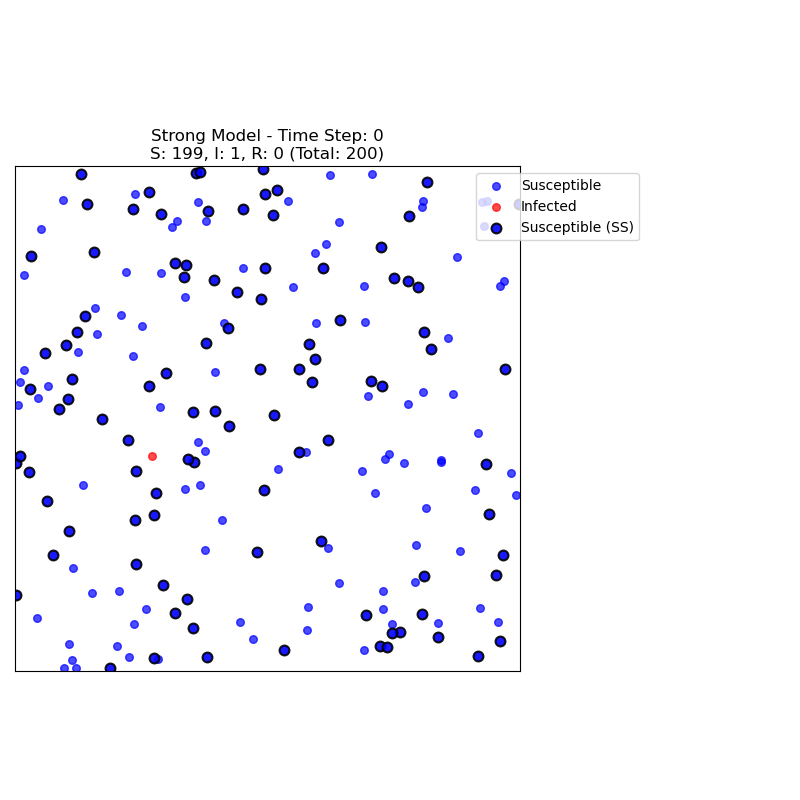
\includegraphics[width=0.4\textwidth]{fig/sir_strong_step_0.png} \\
        Hub Model (Step 0) & Strong Infectiousness Model (Step 0) \\
        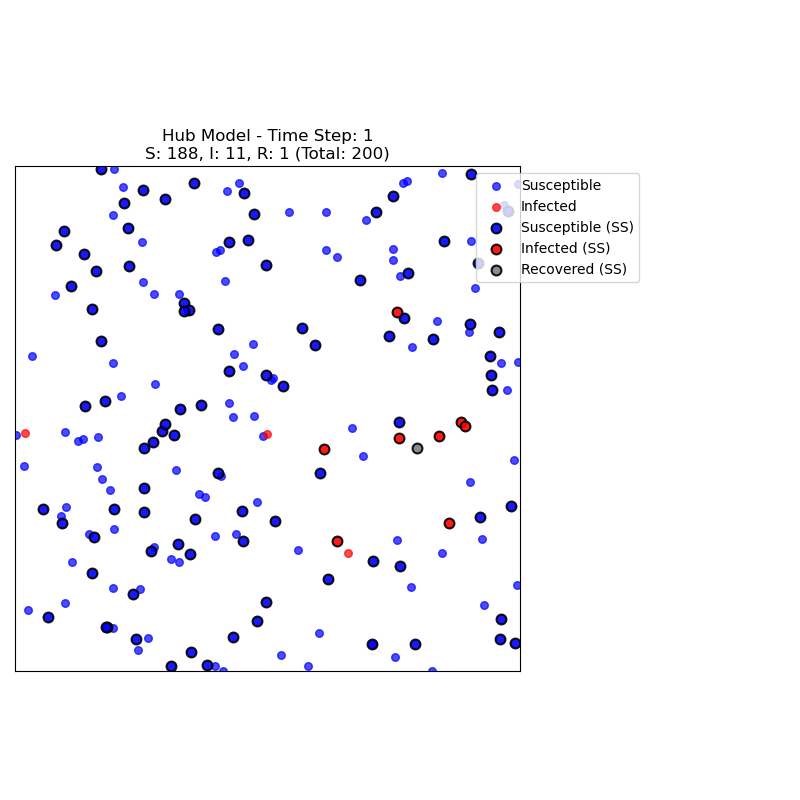
\includegraphics[width=0.4\textwidth]{fig/sir_hub_step_1.png} &
        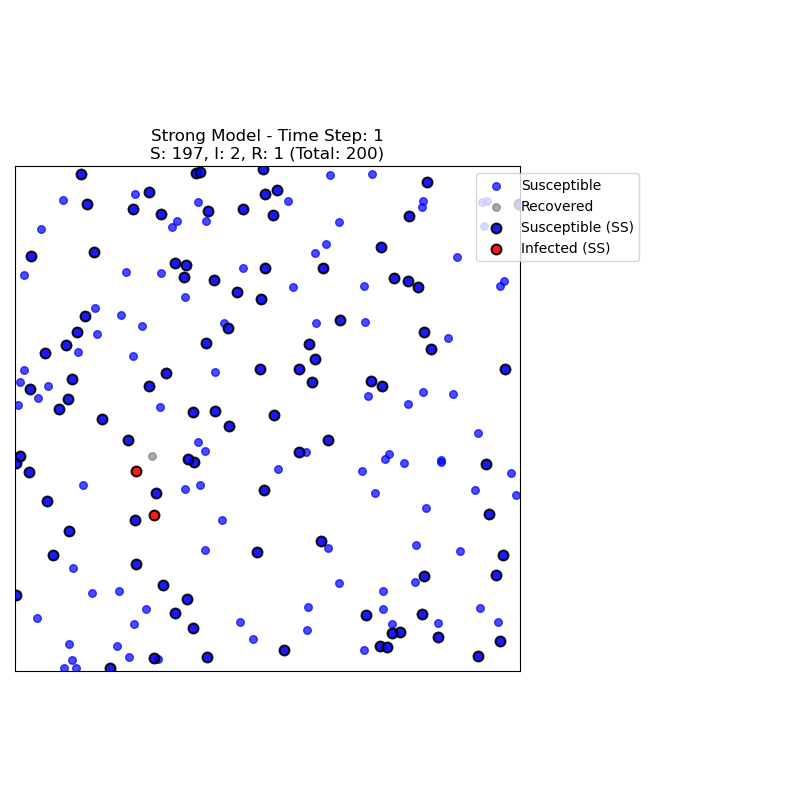
\includegraphics[width=0.4\textwidth]{fig/sir_strong_step_1.png} \\
        Hub Model (Step 1) & Strong Infectiousness Model (Step 1) \\
    \end{tabular}
    \caption{Side-by-side snapshots of the Hub Model (left) and Strong Infectiousness Model (right) at time steps 0 and 1. Blue: Susceptible, Red: Infected, Grey: Recovered. Superspreaders are outlined in black.}
    \label{fig:side_by_side_snapshots_1}
\end{figure}

\begin{figure}[!htbp]
    \centering
    \begin{tabular}{cc}
        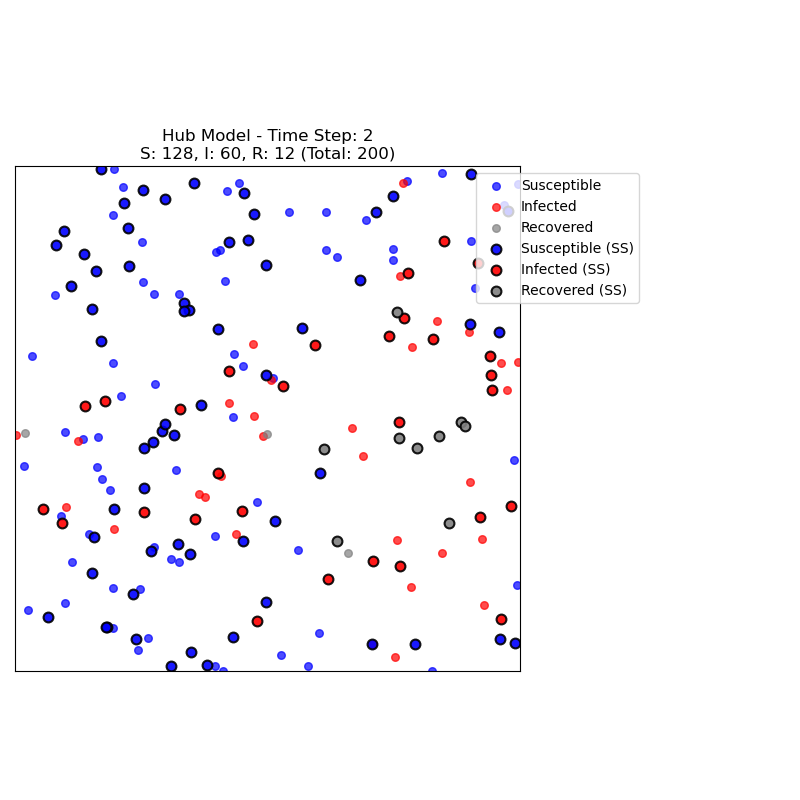
\includegraphics[width=0.4\textwidth]{fig/sir_hub_step_2.png} &
        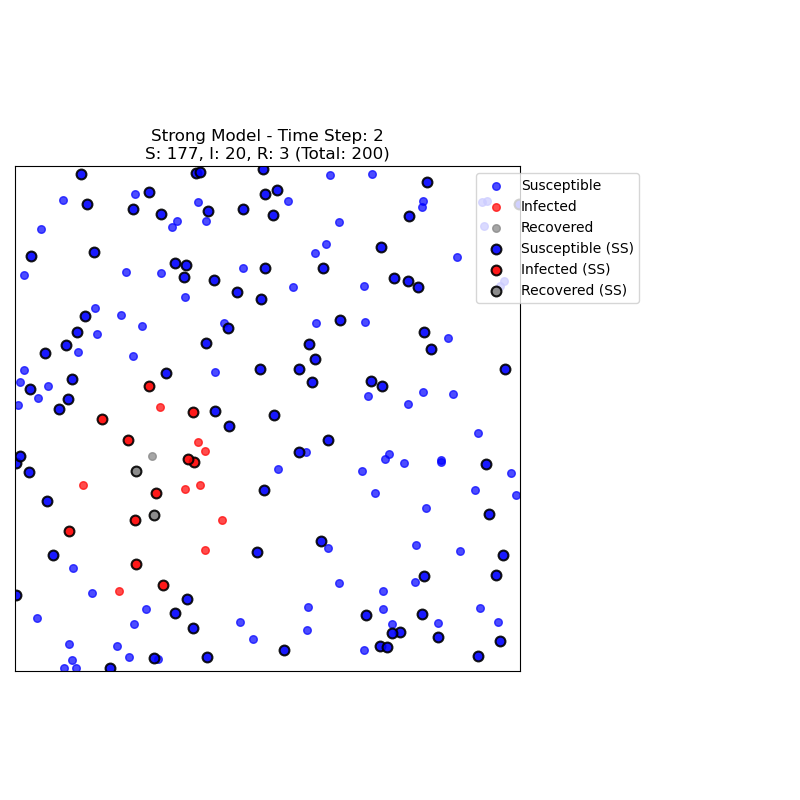
\includegraphics[width=0.4\textwidth]{fig/sir_strong_step_2.png} \\
        Hub Model (Step 2) & Strong Infectiousness Model (Step 2) \\
        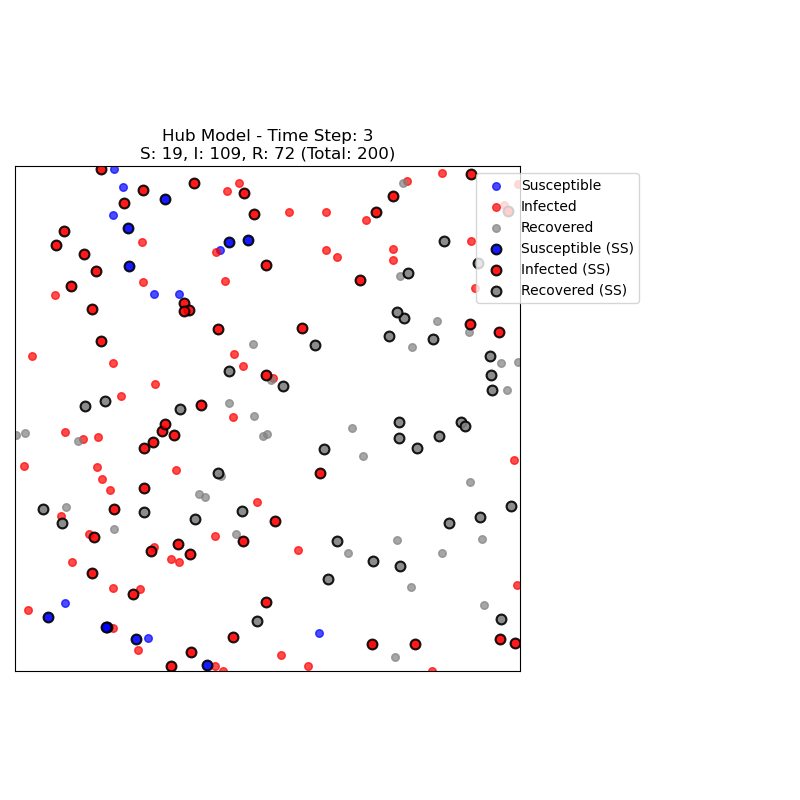
\includegraphics[width=0.4\textwidth]{fig/sir_hub_step_3.png} &
        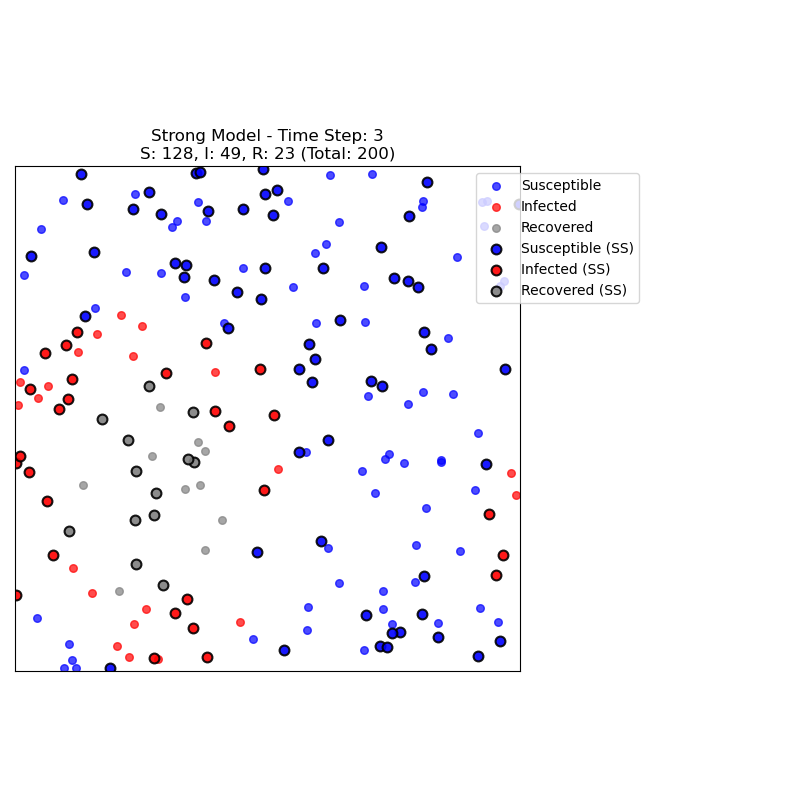
\includegraphics[width=0.4\textwidth]{fig/sir_strong_step_3.png} \\
        Hub Model (Step 3) & Strong Infectiousness Model (Step 3) \\
        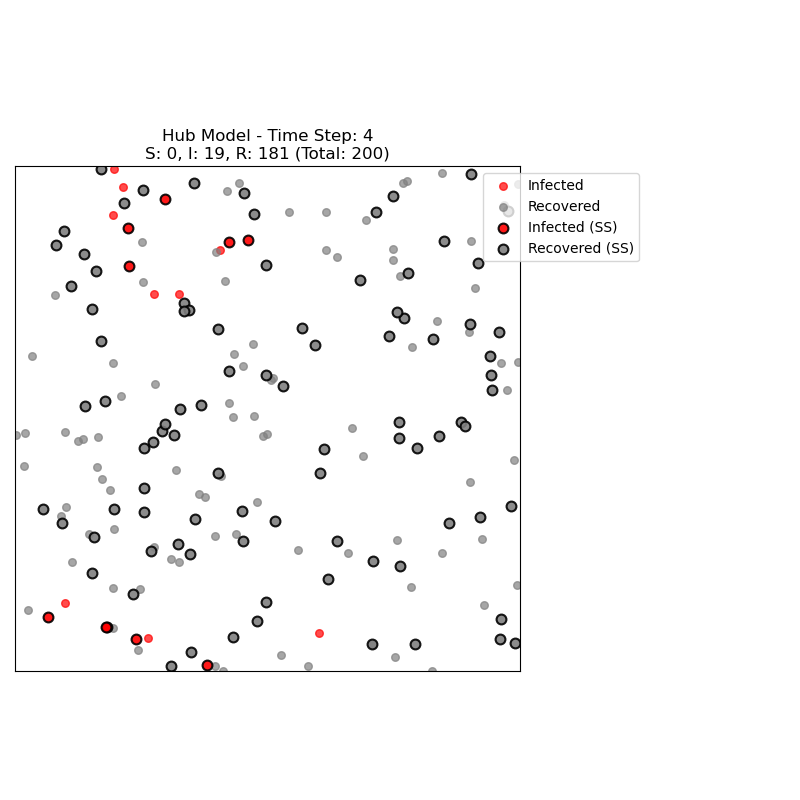
\includegraphics[width=0.4\textwidth]{fig/sir_hub_step_4.png} &
        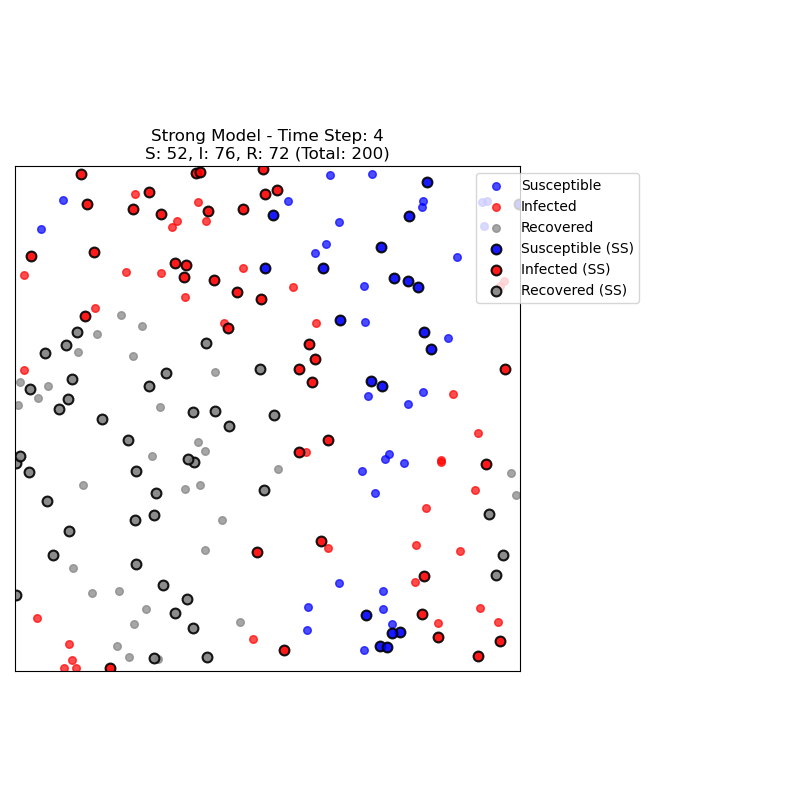
\includegraphics[width=0.4\textwidth]{fig/sir_strong_step_4.png} \\
        Hub Model (Step 4) & Strong Infectiousness Model (Step 4) \\
    \end{tabular}
    \caption{Side-by-side snapshots of the Hub Model (left) and Strong Infectiousness Model (right) at time steps 2 and 4. Blue: Susceptible, Red: Infected, Grey: Recovered. Superspreaders are outlined in black.}
    \label{fig:side_by_side_snapshots_2}
\end{figure}

\begin{figure}[!htbp]
    \centering
    \begin{tabular}{cc}
        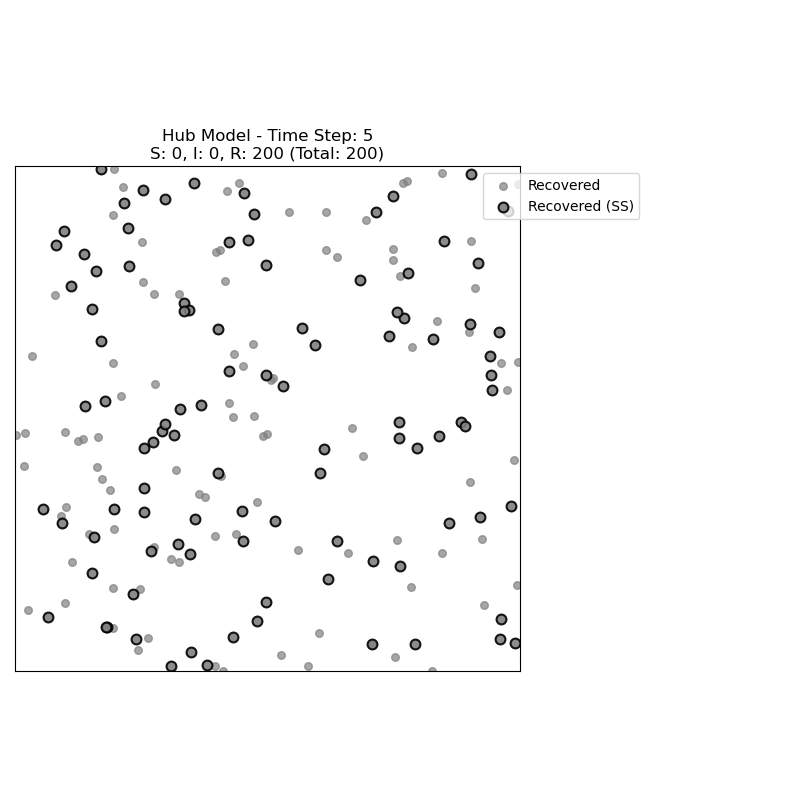
\includegraphics[width=0.4\textwidth]{fig/sir_hub_step_5.png} &
        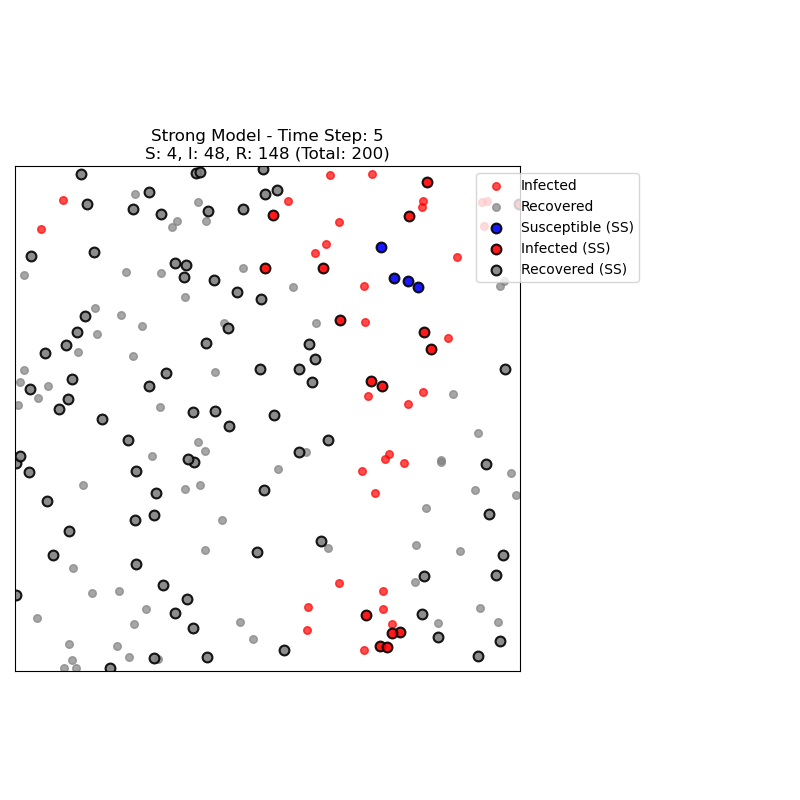
\includegraphics[width=0.4\textwidth]{fig/sir_strong_step_5.png} \\
        Hub Model (Step 5) & Strong Infectiousness Model (Step 5) \\
        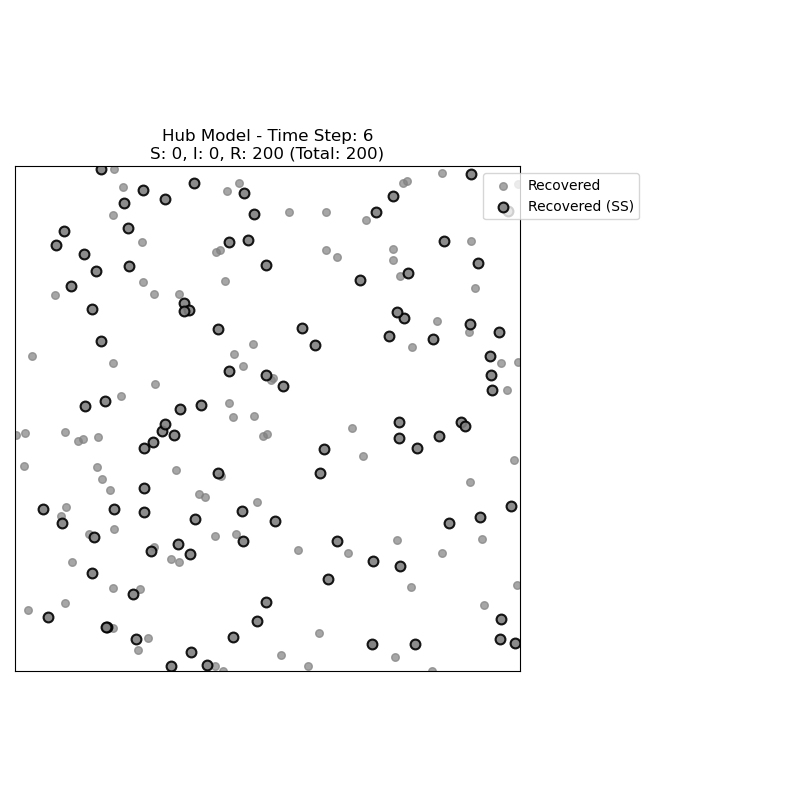
\includegraphics[width=0.4\textwidth]{fig/sir_hub_step_6.png} &
        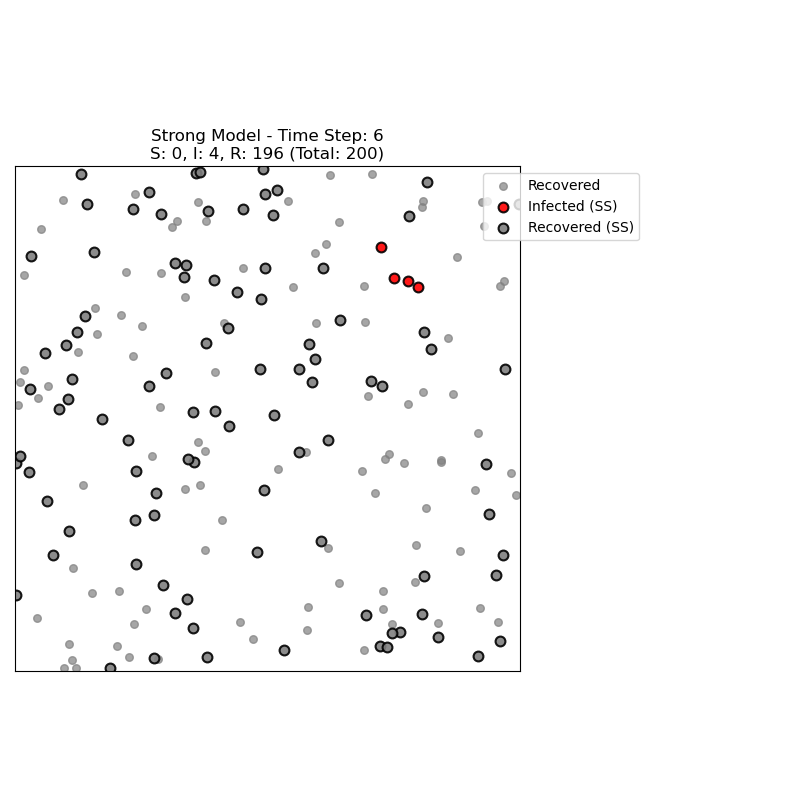
\includegraphics[width=0.4\textwidth]{fig/sir_strong_step_6.png} \\
        Hub Model (Step 6) & Strong Infectiousness Model (Step 6) \\
    \end{tabular}
    \caption{Side-by-side snapshots of the Hub Model (left) and Strong Infectiousness Model (right) at time steps 5 to 6. Blue: Susceptible, Red: Infected, Grey: Recovered. Superspreaders are outlined in black.}
    \label{fig:side_by_side_snapshots_3}
\end{figure}

\subsection{Epidemic curves}

\begin{figure}[!htbp]
    \centering
    \begin{tabular}{cc}
        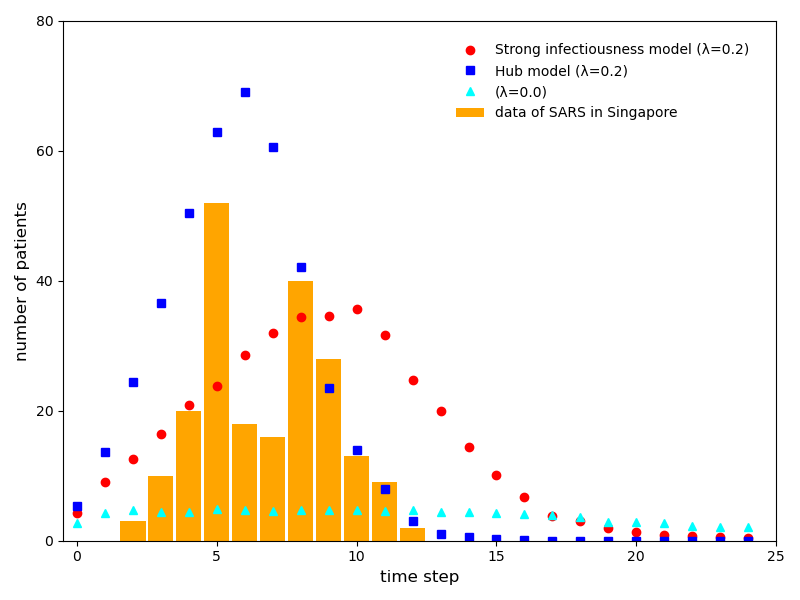
\includegraphics[width=0.9\textwidth]{fig/epidemic_curve.png}
    \end{tabular}
    \caption{Number of patients of both models compare to SARS data from 2003}
    \label{fig:epidemic_curve}
\end{figure}

\end{document}